\textit{I følgende afsnit beskrives den overordnede metode anvendt til besvarelse af problemformuleringen. Denne metode indebærer blandt andet benyttelse af HTA-core modellen og opbygningen af en organiseret søgeteknik. Ligeledes argumenteres der for hvilke dele af HTA-core modellen der er relevante i forhold til besvarelsen af problemformuleringen.}

\section{Projektets metode}
I dette projekt tages udgangspunkt i HTA-core modellen, hvilket afspejles i projektets metode. HTA-core modellen bidrager til at analysere og diskutere de essentielle problemstillinger ved QST, samt at præsentere resultaterne fundet ved analysen og diskussionen \citep{HTAcore}. Ydermere bidrager benyttelsen af HTA-core modellen til en systematisk og bred vurdering af QST. Dette danner et grundlag til beslutningstagning i forhold til eventuel implementering af QST. \citep{metodehaandbogen} \citep{HTAcore} Det er vurderet, at HTA-core modellen bidrager til besvarelse af problemformuleringen, da denne lægger op til en analyse af væsentlige faktorer ved QST, set ud fra et sundhedsvidenskabeligt perspektiv. I projektet inddeles analysen af problemformuleringen i ni forskellige domæner \citep{HTAcore}:

\begin{enumerate}
\item Sundhedsmæssigt problem og nuværende brug af teknologien (CUR)
\item Beskrivelse og tekniske karakteristika for teknologien (TEC)
\item Klinisk effekt (EFF)
\item Sikkerhed (SAF)
\item Organisatoriske aspekter (ORG)
\item Patient- og sociale aspekter (SOC)
\item Etisk analyse (ETH)
\item Juridiske aspekter (LEG)
\item Omkostninger og økonomisk evaluering (ECO)
\end{enumerate}

Inddragelse af HTA-core modellen i projekets opbygning illustreres på \figref{fig:metode}. I dette projekt er domænerne opsat, som det fremgår af rækkefølgen ovenover, men som det ses ud fra \figref{fig:metode}, er der et samspil mellem domænerne. 

\begin{figure}[H] 
	\begin{center}
		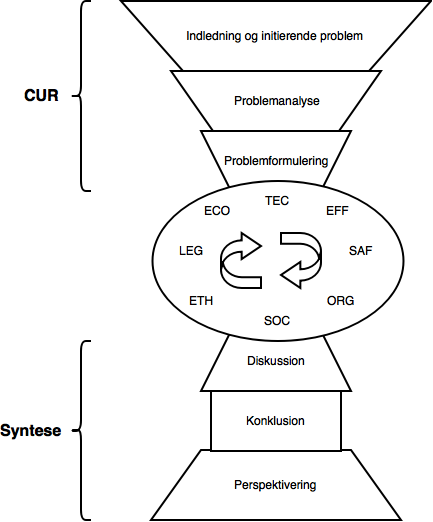
\includegraphics[width=0.5\textwidth]{figures/cMetode/metode}
	\end{center}
	\caption{Figuren viser hvordan HTA-core modellen er blevet inddraget i projektets metode. Det ses, at CUR-domænet er blevet udarbejdet forud for de resterende otte domæner. De otte domæner er udarbejdet separat, men interagerer med hinanden.} 
	\label{fig:metode} 
\end{figure}

Som det illustreres på \figref{fig:metode} ses det, at CUR-analysen er udarbejdet først og på baggrund heraf opstilles en problemformulering. Denne problemformulering er omdrejningspunktet for de resterende domæner og analyse heraf. De otte resterende domæner indgår, nogle mere end andre, i et sammenspil til at besvare problemformuleringen. For at de enkelte analyser af de forskellige domæner kan bidrage til besvarelse af problemformuleringen, bliver de opbygget af netop domæner og analyse-spørgsmål, der tager udgangspunkt i problemformuleringen. For at systematisere analyserne er analyse-spørgsmålene inddelt i emner. Denne kombination kaldes et vurderingselement. Opbygningen af et vurderingselement kan ses på \figref{fig:vurderingselement}. Når et eller flere analyse-spørgsmål under et emne er besvaret, kan besvarelsen af emnet samles med svar fra andre emner i domænet, i en delkonklusion. Delkonklusionerne for de enkelte vurderingselementer sammenfattes til sidst i syntesen for at give et samlet svar på problemformuleringen.\citep{HTAcore}

%Vurderingselementer er en betegnelse for det samlede produkt for analysen af et af de ni områder. Hvert domæne bliver inddelt i emner der hver skal klarlægge et bestemt problem indenfor domænet. Hvert emne specificeres yderligere ved konkrete HTA-spørgsmål, som skal besvares for at kunne besvare problemformuleringen. Når et eller flere HTA-spørgsmål under et emne er besvaret, kan besvarelsen af emnet samles med svar fra andre emner i domænet, i en delkonklusion. Delkonklusionen er besvarelsen af et domæne, og svaret indgår som et vurderingselement til den endelige besvarelse af problemformuleringen. \citep{HTAcore} \Figref{fig:vurderingselement} viser den beskrevne opbygning af vurderingselementet. 

\begin{figure}[H] 
\begin{center}
\includegraphics[width=0.15\textwidth]{figures/cMetode/vurderingselement}
\end{center}
\caption{Opbygningen af et vurderingselement. Figuren viser, hvordan vurderingselementet samlet er udgjort af de tre elementer; område, emne og problematik.}
\label{fig:vurderingselement} 
\end{figure}

I dette projekt opstilles analyseområderne med inspiration fra retningslinjerne i håndbogen for HTA-core modellen. Disse retningslinjer omfatter blandt andet generelle forslag til analyse-spørgsmål, der kan tages udgangspunkt i til de enkelte domæner. Det fremgår desuden, hvilke andre vurderingselementer, domænet relaterer til. Herudover angives det, hvilken metode og hvilken type litteratur, der kan være medvirkende til at besvare analyse-spørgsmålene i et givent domæne. \citep{HTAcore} \\
Afslutningsvis vil de enkelte vurderingselementer og problemformuleringen, sammenfattes i en syntese indeholdende en diskussion af resultater, en konklusion på problemformuleringen samt en perspektivering. 

\subsection{Argumentation for valg af domæner}
Før besvarelse af hvert domæne, argumenteres der for det enkelte domænes relevans for besvarelsen af problemformuleringen. Dette skal sikre, at kun de vurderingselementer der bidrager til besvarelse af problemformuleringen inddrages i projektet. 

Det første domæne, CUR, lægger op til analyse af et sundhedsmæssigt problem og mulige løsninger på problemet. Hermed er domænet relevant for dette projekt, idet det er gennem CUR-domænet det problem som resten af domænerne forsøger at besvare findes. CUR-domænet besvares ved benyttelsen af en AAU-inspireret tilgang. Først indledes projektet med et initierende problem, der lægger op til en bred, alsidig undersøgelse af relevante aspekter for projektet, hvilke undersøges i problemanalysen for at finde et konkret problem, som ønskes besvaret. Igennem analysen bliver det initierende problem undersøgt og afslutningsvis afgrænset, hvormed der kan opstilles en problemformulering. Problemformuleringen definerer det konkrete problem, og besvares igennem de resterende domæner i HTA-core modellen. De første to kapitler (\chapref{introduktion} og \chapref{problemanalysen}), udgør dermed i dette projekt CUR analysen. 

I domænet TEC undersøges den valgte teknologi, både i forhold til oprindelige formål og hvordan teknologien kan anvendes i forhold til det opstillede problem. Idet QST generelt har været anvendt i andre sygdomssammenhænge forud for knæartrose, er der udarbejdet et stort spænd af protokoller og det er således relevant at inddrage TEC-domænet, for at få et indgående kendskab til både den generelle QST og de QST-parametre, som anvendes til undersøgelse af knæartrosepatienter. Ligeledes er et kendskab til QST generelt, teknologiens krav til patienter og brugere samt mulighederne for samspillet mellem QST og klinikeren nødvendige, før det er muligt at analysere flere af de andre domæner. 

Domænet EFF har til formål at analysere en QST-undersøgelser til undersøgelse af knæartrosepatienter i forhold til effektivitet og virkningsgrad. Idet QST-undersøgelser af knæartrosepatienter er et relativt nyt tiltag, vil det være relevant at undersøge, hvor effektive disse undersøgelser er i forhold til sensitivitet og specificitet. Dette domæne er ligeledes en relevant del af projektet idet overvejelser fra området kan inddrages i flere af de andre analyser.   

Ved SAF-domænet undersøges sikkerhedsrisici ved en teknologi. For QST-undersøgelser tilpasset kroniske postoperative smerter tilføres en patient smerte for at vurdere patientens reaktion ud fra forskellige parametre. Hermed kan der være sikkerhedsmæssige risici for patienten, hvilket kan føre til eventuelle skader. Det er dermed relevant at undersøge om de undersøgelsesmetoder der anvendes i QST kan skade patienten samt i hvilket omfang dette kan ske. Dette gør det muligt at vurdere hvorvidt de sikkerhedsmæssige risici ved QST-undersøgelserne overgår den diagnostiske relevans for undersøgelserne. 

ORG-domænet har til formål at undersøge konsekvenserne ved de organisatoriske ændringer der vil følge ved implementeringen af QST. Idet QST skal implementeres på en hospitalsafdeling er det betydeligt at vurdere hvor i behandlingsforløbet en sådan implementering er hensigtsmæssig, og i hvilket omfang den nuværende arbejdsgang og kommunikation på afdelingen påvirkes ved brugen af QST. Ligeledes er det organisatoriske aspekt en essentiel del i forhold til en besvarelse af problemformuleringen idet det organisatoriske skal danne ramme for brugen af QST.

I SOC-domænet analyseres problematikker forbundet med patienten og sociale aspekter. Idet QST-undersøgelserne er en teknologi som udføres på hospitalet, hvormed der ingen sociale aspekter ved implementeringen og brugen af QST-undersøgelserne. Det er herimod relevant at undersøge patientaspekterne ved QST-undersøgelserne i forhold til om  der er forhold som kan betyde, at nogle patienter ikke vil kunne få en QST, og i hvilket omfang implementeringen af QST-undersøgelserne påvirker patienten.

Ved ETH-domænet undersøges de etiske aspekter ved en teknologi. Resultatet af at QST skal anvendes som supplement til vurderingsgrundlaget forud for en operation vil det have etiske konsekvenser, hvis QST ikke kan identificere alle patienter med forhøjet risiko for udvikling af kroniske postoperative smerter. Disse overvejelser vil både gælde for falsk positive og falsk negative resultater. Herudover kan der være etiske overvejelser forbundet med, hvilken betydning det vil have at der udføres en HTA på nuværende tidspunkt.         

I LEG-domænet analyseres de love og regulativer der kan være relevante ved implementeringen af en teknologi. QST vil, ligesom alle andre teknologier, som anvendes i sundhedssystemet, være underlagt en række love og regulativer, som kan være afgørende for om hvorvidt anvendelse af teknologien kan tillades. Det vil på baggrund af de andre analyser blive undersøgt om QST overskrider nogle love, og hvordan dette fremgår. 
Det bliver imidlertid fundet i SAF-, SOC- og ETH-analyserne, at QST hverken har sikkerhedsmæssige risici eller påvirker patientaspekter der overskrider love eller etiske retningslinjer. Det eneste aspekt som kan tages til overvejelse er godkendelse fra Etisk Råd. Rådet skal godkende undersøgelser hvor patienten påvirkes på den ene eller anden måde. Da QST vil påføre patienter et mekanisk tryk, skal rådet derfor kontaktes og godkende undersøgelsen. Dette anses dog ikke som en forhindring, da risici ved QST-undersøgelser er minimale, jævnfør SAF-analysen, og derfor vil blive godkendt af Etisk Råd. 
Der fremgår således ingen tydelige problemstillinger ved overholdelse af love, hvorved det ikke anses for relevant at analysere dette domæne, da analysen ikke vil kunne bidrage til besvarelse af problemformuleringen.

I ECO-domænet undersøges problemet ud fra et økonomisk synspunkt. Da det for QST-undersøgelserne er nødvendigt at anvende teknologisk udstyr, er der omkostninger forbundet med implementering af disse. Ligeledes vil der blandt andet være omkostninger ved oplæring af personale. Disse økonomiske omkostninger sættes op imod gevinster ved implementeringen af QST. Disse gevinster kan være både monetære eller tage anden form. Det er relevant at undersøge implementeringen og brugen af QST ud fra et økonomisk perspektiv, for at beslutningstagere kan vurdere, om de økonomiske udgifter er acceptable i forhold til udbyttet af implementeringen af QST til undersøgelse af knæartrosepatienter. 

\subsection{Litteratursøgning} \label{litteratursogning}
Litteratursøgning og -vurdering i projektet tager udgangspunkt i retningslinjerne opstillet i Metodehåndbogen for Medicinsk Teknologivurdering udarbejdet af Sundhedsstyrelsen \citep{metodehaandbogen}. Da projektet udarbejdes på baggrund af videnskabelig litteratur, er det væsentligt, at litteraturen findes og vurderes ved en organiseret fremgangsmåde, således at problemformuleringen besvares på et veldokumenteret grundlag. Litteratursøgningen vil derfor være den samme for alle domæner i rapporten. For hvert domænes metode vil litteratursøgning kun beskrives i så fald søgningen for det specifikke område afviger fra den generelle litteratursøgningsmetode som beskrevet her. \\
Generelt for litteratursøgning vil der blive søgt på sundhedsvidenskabelige databaser som: PubMed, MEDLINE, EMBASE og Cochrane Library. Aalborg Universitetsbiblioteks søgemaskine Primo vil ligeledes tages i brug og anvendes som generel søgeværktøj, da denne dækker flere databaser. For ligeledes at sikre ensartethed gennem rapporten vil udvælgelsen og vurderingen af litteratur forløbe efter samme søgestrategi for alle domæner. Søgestrategien bygger på anvendelse af relevante søgetermer og explicitte søgekriterier, så som AND, OR, NOT og *.  De specifikke søgetermer er lavet på baggrund af en brainstorm over spørgsmålet, således flest mulige inputs blev taget i betragtning. Herved blev der valgt nogle søgeord som, under søgeprocessen er blevet optimeret løbende. Ved anvendelse af disse termer og kriterier er det forsøgt at bringe antallet af hits per søgning på under 100 hits. Herefter er alle overskrifter for den pågældende søgning blevet gennemgået for relevans. Ved litteratur som ud fra overskriften vurderes relevant, er abstract efterfølgende blevet gennemlæst for at sortere materialet. Litteratur som efter gennemlæsning af overskrift og abstract er vurderet som værende relevant for besvarelsen af analyse-spørgsmålet er blevet læst, vurderet ud fra evidensniveau og anvendt til besvarelse af analyse-spørgsmålet. Noget litteratur er fundet gennem snowballing, hvor litteratur findes gennem referencelisten for andet litteratur. \\ 
Søgestragtegien for de enkelte domæner er dokumenteret i en søgeprotokol. Søgeprotokollen har ligeledes til formål at gøre det muligt for interessenter at forstå, hvordan litteratursøgningen er forløbet. \citep{metodehaandbogen} Til at udarbejde søgeprotokollen i dette projekt, er der opstillet en skabelon, der systematiserer litteratursøgningen. Et uddrag af skabelonen ses i \figref{fig:soegeprotokol}.

\begin{figure}[H]
\begin{center}
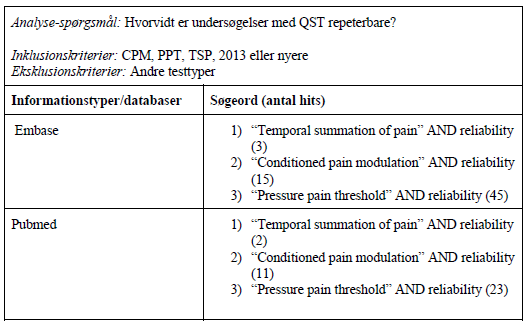
\includegraphics[width=0.5\textwidth]{figures/cMetode/spex}
\end{center}
\caption{Figuren viser en skabelon for projektets søgeprotokol. Det fremgår af skabelonen, at der for hver søgning inddrages ét analyse-spørgsmål samt inklusions- og eksklusionskriterier. Ligeledes dokumenteres det, hvilke databaser, der er anvendt til søgningen. For hver database opstilles de specifikke søgeord, og antallet af hits fremgår i parentesen herefter. Eksemplet viser, at de benyttede søgeord tager udgangspunkt i analyse-spørgsmålet. De tre QST-parametre der ønskes undersøgt er benyttet sammen med den engelske oversættelse af repeterbarhed.}
\label{fig:soegeprotokol} 
\end{figure} \vspace{-.25cm}

Analyse-spørgsmålene for de enkelte domæner anvendes i søgeprotokollen til at definere, hvad der ønskes svar på ved de enkelte søgninger. Søgeordene fastsættes på baggrund af de enkelte analyse-spørgsmål ved at uddrage de væsentlige aspekter fra hvert spørgsmål og hermed sammensætte søgningen.\\ %der har til formål at bidrage til besvarelsen af problemformuleringen indenfor de otte domæner. Spørgsmålene er afgrænsede og entydige, således at det er muligt at finde konkret litteratur til besvarelse af disse. \citep{metodehaandbogen}  \\
For at afgrænse og sikre relevansen af søgeresultaterne, opstilles inklusions- og eksklusionskriterier for søgningerne. Søgningerne kan eksempelvis afgrænses til kun at indeholde bestemte typer studier, en eller få specifikke sygdomme, en afgrænset aldersgruppe med mere. \citep{metodehaandbogen} \\
Dokumentationen af valgte databaser samt tilhørende søgeord er en væsentlig del af søgeprotokollen, da databaserne har forskellige typer syntaks til litteratursøgning, hvormed det er vigtigt, at søgningen i en given database er foretaget med anvendelse af søgetermerne specifikke for den valgte database. \citep{metodehaandbogen}

\subsubsection{Evidenshieraki}
Litteraturen i dette projekt inddeles ud fra evidenshierakiet i \citer{metodehaandbogen}. Evidenshierakiet omfatter følgende syv punkter, hvor kilder med det højeste evidensniveau er placeret øverst i listen:

\begin{enumerate}
\item Metaanalyser og systematiske undersøgelser 
\item Randomiserede kontrollerede undersøgelser (RCT’s)
\item Ikke-randomiserede kontrollerede undersøgelser
\item Kohorte undersøgelser
\item Case-kontrol undersøgelser
\item Deskriptive undersøgelser, mindre serier
\item Konsensusrapporter, ikke-systematiske oversigtsartikler, ledere, ekspertudtalelser
\end{enumerate}

Metaanalyser og systematiske undersøgelser er sekundær litteratur og har det højeste evidensniveau. Denne type litteratur er statiske sammenfatninger af primær litteratur med samme afgrænsede problemstilling. \citep{denstoredanske2009} \\
Randomiserede kontrollerede undersøgelser (RCT) er primær litteratur, hvor der foretages en sammenligning af to forsøgsgrupper. Den ene gruppe udsættes for en påvirkning, mens den anden gruppe fungerer som kontrolgruppe. Udvælgelsen af forsøgspersoner foregår tilfældigt. \citep{denstoredanske2009a} \\
Ikke-randomiserede kontrollerede undersøgelser er ligesom RCT’s primær litteratur, hvor to forsøgsgrupper sammenlignes. Ved disse undersøgelser sker udvælgelsen af forsøgspersoner ikke tilfældigt, hvormed evidensniveauet falder da der ikke på samme måde som ved RCT tages højde for bias i forsøgsgrupperne. \citep{denstoredanske2009a} \\
Ved kohorte undersøgelser følges flere forsøgsgrupper over en periode for at undersøge, hvorvidt bestemte eksponeringer har indflydelse på udviklingen af helbredsfænomener, herunder sygdom og død. \citep{metodehaandbogen} \\
I case-kontrol undersøgelser, forsøges det at undersøge forskellige faktorers indflydelse på udvikling af bestemte sygdomme. Dette gøres ved en sammenligning mellem en forsøgsgruppe med den pågældende sygdom og en forsøgsgruppe bestående af raske personer. I modsætning til eksempelvis kohortestudiet følges forsøgsgrupperne ikke over tid, hvormed der ikke kan udføres en opfølgende undersøgelse. Det er således ikke muligt at estimere betydningen af  risikofaktorerne. \citep{denstoredanske2012} \\
Deskriptive studier er studier hvor der foretages analyser til beskrivelse af et fænomen. I modsætning til de andre typer studier påvirkes forsøgsgrupperne ikke. I stedet undersøges nuværende tendenser, eksempelvis med henblik på senere udførelse af et forsøg. \citep{} \\
Fælles for gruppen af konsensusrapporter, ikke-systematiske oversigtsartikler samt ledere og ekspertudtalelser er, at materialet oftest er udtryk for subjektive holdninger, der ikke er underbygget af tilstrækkelige mængder supplerende litteratur, der undersøger området. \citep{metodehaandbogen} \\
Alt litteratur anvendt i dette projekt vurderes ud fra evidenskierakiet. Evidensen for litteraturen er angivet i litteraturlisten med et nummer der svarer til nummeret for hver af de syv evidensniveauer.   